\documentclass[journal]{IEEEtran}
\usepackage{amsmath,amssymb,booktabs,cite,graphicx,placeins}
\usepackage[hidelinks]{hyperref}
\newif\ifnativecases
\ifdefined\NativeCaseReview\nativecasestrue\else\nativecasesfalse\fi
\newcommand{\CaseAsset}[2]{\ifnativecases local_figures/#2\else figures/journal_20261126/#1\fi}
\newcommand{\MethodAsset}[1]{\ifnativecases local_method_figures/#1\else figures/method_atlas_20261126/#1\fi}
\newcommand{\ObservedMethod}[1]{\ifnativecases local_observed_figures/#1\else figures/observed_methods_20261127/#1\fi}
\newcommand{\ObservedCase}[1]{\ifnativecases local_observed_figures/#1\else figures/observed_cases_20261127/#1\fi}
\DeclareRobustCommand{\CaseCaption}[2]{\ifnativecases #2\else #1\fi}
\hypersetup{pdftitle={NORA: Native-Grid Occupancy Ranking and Allocation for SAR Ship Instance Segmentation}}
\begin{document}
\raggedbottom
\title{NORA: Native-Grid Occupancy Ranking and Allocation for SAR Ship Instance Segmentation}
\author{Author~Details~Pending\thanks{Author affiliations and submission metadata are pending.}}
\maketitle

\begin{abstract}
A ship detector can locate a narrow vessel in a synthetic aperture radar (SAR) image yet assign foreground to the wrong side of its hull. Native-Grid Occupancy Ranking and Allocation (NORA) refines the binary mask of a retained detection. A residual head learns the fraction of each boundary cell covered by a ground-truth polygon. With the numbers of additions and removals fixed, NORA ranks the two sets of cells independently. With only the total count fixed, a separately fitted head predicts foreground membership under two raster references and guides the split between additions and removals. Independent selection improves mask average precision (AP) by 0.81--0.91 points over distance-first pairing across three detector configurations on HRSID DEV705. On the same 74 historical Instance-RSDD reserve chips, its gain over re-pairing within the original distance limit is 0.479 points with RF-DETR and 0.344 with D-FINE. Re-pairing within the distance limit improves one-pixel Boundary IoU by 0.735 points over distance-first pairing with RF-DETR. The paired 95\% interval for the additional change in Boundary IoU under independent selection spans zero. Compared with an equal split, variable allocation gains 2.30 and 1.75 AP points under two annotations of the same SSDD images, averaged over three head fits. On frozen transfer to SAR-SSP, it recovers missed foreground but adds excess foreground, and AP falls by 0.14 points.
\end{abstract}
\begin{IEEEkeywords}
Synthetic aperture radar, ship instance segmentation, mask refinement, boundary supervision.
\end{IEEEkeywords}

\section{Introduction}
\label{sec:introduction}

A ship moored alongside a quay can be easy to locate in a synthetic aperture radar (SAR) image even when its outline is difficult to trace. SAR records coherent returns from the scene~\cite{moreira2013}. A bright return may come from a scattering structure inside the hull or from a neighboring structure on shore~\cite{gao2024,gldet}. A predicted box can therefore enclose the right ship while its mask omits a strip of hull on one side and extends onto the quay on the other. Correcting this error requires deciding what the image and mask tell us about each boundary cell, where to change the mask, and whether its foreground area should change.

First, an annotated outline can cross a cell whose center lies outside the polygon. Adding this cell to the mask contributes a fraction of its area to the intersection, although its center label assigns it entirely to the background. Native-Grid Occupancy Ranking and Allocation (NORA) uses the fraction covered by the reference polygon as a training target. A residual occupancy head (ROH) combines the detector response with local mask geometry and image appearance to estimate this fraction. This defines occupancy relative to the annotated hull on the native image grid.

Second, a mask with the right area can still have poor overlap. Moving a four-cell-wide rectangular hull sideways by one cell leaves its area unchanged but reduces its intersection over union (IoU) to $3/5$. An addition at the missing flank and a removal at the opposite flank can restore overlap. Requiring those edits to be close can rule out that choice. NORA compares distance-first pairing, re-pairing within the same maximum distance, and independent ranking of additions and removals. Each rule uses the same occupancy estimates and changes the same number of cells on each side. The comparison tests how much the pairing requirement restricts placement.

Third, a mask that misses a strip of hull and has little excess foreground needs a net increase in area. Equal numbers of additions and removals preserve the deficit wherever the edits are placed. NORA therefore allows their relative numbers to vary while holding their sum fixed. When two annotation releases describe the same training image, a dual-reference head estimates the probability that a cell belongs to the ship under each reference. The allocation favors edits with a predicted overlap gain under both references. Across these decisions, NORA returns the refined binary mask with the original detection identity, box, class and confidence.

\section{Related Work}
\label{sec:related-work}

\subsection{SAR mask geometry and fractional occupancy}
The outlines in HRSID and the polygon subset of SSDD made it possible to evaluate SAR ship masks at finer spatial detail than a detection box affords~\cite{hrsid,ssdd}. Boundary IoU further distinguishes agreement along a narrow contour band from overlap over the whole instance~\cite{boundaryiou}. One approach to recovering ship contours is to align the prediction region with the hull. SRNet predicts masks inside rotated boxes, and DRSNet uses dual-scale cross-attention within rotated regions~\cite{rsdd,drsnet}. Other methods draw on the imaging characteristics of SAR. Gao \emph{et al.} associate scattering responses with individual ships through dynamic key points~\cite{gao2024}. GLDet combines global context with local gradient features~\cite{gldet}. More recent work aligns semantic and boundary representations, uses geometry-aware proposals and multiscale feature fusion, or combines differential features with graph reasoning~\cite{aranet,dacf,dsr}.

These approaches improve the features or spatial region from which a mask is predicted. A retained mask poses a more specific question. When its annotated outline cuts across a native cell, how much intersection area would that cell contribute if assigned to the ship? A binary center label loses this distinction. NORA directly supervises an occupancy estimate with the polygon--cell intersection fraction and uses it to rank candidate edits.

\subsection{Endpoint placement at equal edit counts}
Atkinson used spatial attraction to exchange subpixel labels while preserving the class proportions of each coarse remote-sensing pixel~\cite{atkinson}. Later mask refiners chose locations according to the evidence needed at a boundary. PointRend queries uncertain points as it subdivides a mask, SegFix transfers reliable interior labels to boundary locations, and Boundary Patch Refinement predicts local corrections from image and mask patches~\cite{pointrend,segfix,bpr}. These methods motivate selective boundary updates, but their output differences can reflect changes in the scores, the sites receiving them, and the number of labels that change.

For a retained ship mask, the unresolved issue is whether a promising addition must have a nearby partner for removal. NORA compares choices on the same eligible cells, using the same scores and the same realized number of edits on each side. Allowing new pairs within the original distance limit tests the effect of partner choice. Removing that limit then tests the additional effect of selecting the two sides independently. Total displacement and mask connectivity can vary in both comparisons.

\subsection{Signed allocation at a fixed total count}
RankSEG chooses a foreground count and a prefix of ranked posterior scores to optimize a segmentation overlap criterion~\cite{rankseg}. SegRefiner approaches an existing mask as the starting point for learned discrete denoising updates~\cite{segrefiner}. RankSEG-RMA subsequently made overlap-based ranking more efficient by approximating the reciprocal moment used in binary IoU~\cite{rankrma}. Phoenix learns semantic-aware correction of a whole mask~\cite{phoenix}. A chosen final area is compatible with many different numbers of changes to an input mask. Conversely, requiring equal additions and removals preserves the input area even when that area is wrong.

NORA asks how to divide a prescribed number of changes between the two signs. It uses the RankIoU-RMA overlap estimate to compare proposed allocations on the same eligible cells. The equal-split control and the variable-split rule share the same scores, total count and objective. Where two references are available, that objective rewards the smaller predicted overlap gain relative to the same starting allocation. The comparison thus tests the value of redistributing a fixed number of edits under the supplied annotations.

\section{Method}
\label{sec:method}

NORA takes one retained ship detection as input and returns a binary mask on the original image grid (Fig.~\ref{fig:network-overview}). A frozen RF-DETR~\cite{rfdetr} or D-FINE-seg~\cite{dfine} supplies the mask \(M\), box \(B\), class, confidence \(s\) and foreground response \(p_i\) at each sampled cell center. The decoded image supplies local intensity. Only the labels of selected cells can change. Each detection retains its identity, box, class and confidence, and the output stream includes every input candidate, including those ineligible for editing. We use two budgets. Requiring equally many additions and removals preserves each mask's area while the edit locations vary. Fixing their sum also lets the predicted area change.

\begin{figure*}[!t]
\centering
\includegraphics[width=\textwidth]{\MethodAsset{nora_network_overview.pdf}}
\caption{NORA for one retained detection. \CaseCaption{The Sentinel-1A VV image shows the \emph{Ever Given} on 25 March 2021. The \(32\times28\) display averages \(2\times2\) samples of backscatter brightness after clipping to \([-8,10]\) dB. Contains modified Copernicus Sentinel data (2021), terrain-corrected by Catalyst via Microsoft Planetary Computer (\href{https://creativecommons.org/licenses/by/4.0/}{CC BY 4.0}).}{The SAR input shows an Instance-RSDD Gaofen-3 ship before the prediction and reference contours are overlaid.} The network and output mask are schematic. The frozen detector supplies the binary mask \(M\), cell-center response \(p_i\) and detection metadata. The scalar residual occupancy head (ROH) ranks cells for \(F,L,I\) at equal addition and removal counts. A separately fitted dual ROH supplies foreground probabilities for fixed-total allocation. Scalar supervision uses ground-truth polygon--cell fractions. Dual supervision uses foreground labels from two matched raster references.}
\label{fig:network-overview}
\end{figure*}

\subsection{Native boundary sites and residual occupancy}
\label{sec:occupancy}

Let \(\Omega\) denote the decoded \(W\times H\) grid and \(C_i=[x,x+1)\times[y,y+1)\) the unit square at \(i=(x,y)\). We identify \(M\) with the union of its foreground cells. For \(32\le |M|<1024\), we search a two-cell band on each side of its boundary. With dilation \(\delta\) and erosion \(\varepsilon\) using a \(3\times3\) square and zero exterior, the two pools inside the detection box are
\begin{equation}
\begin{aligned}
 \mathcal B_+ &= (\delta^2(M)\setminus M)\cap B\cap\Omega,\\
 \mathcal B_- &= (M\setminus\varepsilon^2(M))\cap B\cap\Omega .
\end{aligned}
\label{eq:native-bands}
\end{equation}
We sort each pool by \((|p_i-\tfrac12|,yW+x)\), giving priority to responses nearest the decision threshold and resolving ties in row-major order. The first \(n=\min(32,|\mathcal B_+|,|\mathcal B_-|)\) cells on each side form the candidate sets \(S_+\) and \(S_-\) (Fig.~\ref{fig:occupancy-stage}). The binary value in \(M\) determines whether a cell may be added or removed, even when its center response lies on the opposite side of 0.5. Masks outside the area range and masks with an empty pool pass through unchanged.

\begin{figure}[!t]
\centering
\includegraphics[width=\columnwidth]{\ObservedMethod{observed_sampling.pdf}}
\caption{Native boundary support. Within the box \(B\), the writer takes candidate additions from the outer two rings and removals from the inner two rings. Candidates on each side are ordered by \(\lvert p_i-0.5\rvert\) and capped at 32. \CaseCaption{The top panels use a schematic mask, box and scores. The lower panel shows a D-FINE native mask on the Instance-RSDD reserve, pooled into \(8\times8\) display bins and rounded to quarter occupancy. Its native continuous IoU is 51.71 points.}{The left panel shows the observed D-FINE mask on the Instance-RSDD reserve. The displayed box and score ordering illustrate the sampling rule.}}
\label{fig:occupancy-stage}
\end{figure}

The ROH scores each candidate cell from its decoder response, mask geometry, detection attributes and local appearance. Its input has 14 components,
\begin{equation}
\begin{aligned}
 v_i=\bigl(&p_i,M_i,\ell_i,d_i,\bar x_i,\bar y_i,\nu,\eta,s,\\
           &L_i,\bar L_{3}(i),\bar L_{5}(i),\Delta_x L_i,\Delta_y L_i\bigr)^{\!\top}.
\end{aligned}
\label{eq:endpoint-features}
\end{equation}
Here \(M_i\) is the binary label, \(\ell_i\in\{1,2\}\) is the ring index, \(d_i\) is the Euclidean distance to the opposite binary class, and \((\bar x_i,\bar y_i)\) gives the box-normalized position. Distances use native pixels and areas use unit cells. Mask size \(\nu=\log_2|M|\), box fill \(\eta=|M|/|B\cap\Omega|\) and detection confidence \(s\) are shared within a candidate. The last five components describe appearance in the released image rendering. They comprise cell intensity, its \(3\times3\) and \(5\times5\) neighborhood means, and its horizontal and vertical central differences. At the cell center, D-FINE interpolates the stored sigmoid response bilinearly. RF-DETR interpolates the logits before applying the sigmoid. Supplementary Section~S1 specifies the half-cell coordinates, padding and numerical precision.

Training requires a source detection with a nonignored COCO match at raster IoU 0.50 and a valid ground-truth polygon \(G\). For a cell crossed by the annotated contour, a center label discards the extent of coverage. The scalar head therefore uses the fraction
\begin{equation}
 q_i=|C_i\cap G|/|C_i| .
 \label{eq:fractional-target}
\end{equation}
Thus \(q_i\) measures coverage by the released annotation, while \(p_i\) samples the detector response at a point (Fig.~\ref{fig:fractional-readout}). At inference, predicted coverage ranks possible edits. Each selected cell still receives a binary label on the native grid.

\begin{figure*}[!t]
\centering
\includegraphics[width=\textwidth]{\ObservedMethod{observed_readout.pdf}}
\caption{Target and decoder response for the scalar ROH. \CaseCaption{At left, the Instance-RSDD reference polygon is pooled into an \(8\times8\) display grid with quarter-occupancy levels.}{At left, the annotated outline is overlaid on the Instance-RSDD SAR crop.} The other panels illustrate one native cell. The polygon covers half of this example cell (\(q_i=0.50\)). Bilinear interpolation of four decoder neighbors gives \(p_i\) at the same cell center.}
\label{fig:fractional-readout}
\end{figure*}

We standardize \(v_i\) to \(z_i\) using statistics that weight the training source groups equally. The ROH learns a correction to the decoder logit,
\begin{equation}
 \begin{aligned}
 \widehat q_i&=\operatorname{sigmoid}
  \bigl(\operatorname{logit}(p_i^\epsilon)+f_\theta([z_i,z_i])\bigr),\\
 p_i^\epsilon&=\operatorname{clip}(p_i,10^{-4},1-10^{-4}) .
 \end{aligned}
 \label{eq:occupancy-head}
\end{equation}
The network \(f_\theta\) (Fig.~\ref{fig:roh-architecture}) has widths \(28\to24\to24\to1\), two ReLU activations and 1,321 parameters. Both copies of \(z_i\) describe the same cell. This matches the input width of a control that also receives a partner's features. Initializing the final affine layer to zero gives \(\widehat q_i=p_i^\epsilon\) before fitting. We draw source groups uniformly, then sample a pair \((a_j,d_j)\) within each selected group. For \(m\) pairs the loss is
\begin{equation}
 \mathcal L_{\mathrm{occ}}=
 \frac{1}{2m}\sum_{j=1}^m\bigl[
 \ell(q_{a_j},\widehat q_{a_j})+\ell(q_{d_j},\widehat q_{d_j})\bigr],
 \label{eq:occ-loss}
\end{equation}
where \(\ell(q,p)=-q\log p-(1-q)\log(1-p)\). We fit the scalar ROH with 200 AdamW updates of 64 pairs, learning rate \(0.002\) and weight decay \(0.01\). FIT109 contains 109 HRSID fitting chips, one per filename-prefix group, from the detector fitting population. In each cross-fitting fold, the held-out prefixes contribute neither examples nor scaling statistics to the ROH fit. For transfer we fit the head and its scaling on all of FIT109 and freeze both.

\begin{figure*}[!t]
\centering
\includegraphics[width=\textwidth]{\MethodAsset{nora_roh_architecture.pdf}}
\caption{ROH at one candidate cell. The four feature groups contain 4, 2, 3 and 5 components. The head concatenates two copies of the standardized vector. Matrix dimensions are output by input, and each affine layer has a bias. The scalar and dual heads are fitted separately. Both add residuals to the clipped decoder logit and use binary cross-entropy. The scalar target \(q_i\) is a GT polygon--cell area fraction. The dual targets \((y_{i1},y_{i2})\in\{0,1\}^2\) are the foreground labels of the matched ship under two raster references. The final affine layer is initialized to zero.}
\label{fig:roh-architecture}
\end{figure*}

\subsection{Placement at equal signed counts}
\label{sec:selection}

For a given mask, all three placement rules receive the same \(S_+\), \(S_-\) and ROH scores. Distance-first pairing (\(F\)) first matches the full lists one to one to minimize total squared distance on the native grid. It then ranks these pairs by \(\widehat q_a-\widehat q_d\), breaking ties by the addition's row in the list. It keeps pairs with positive estimated gain up to \(K=\min(8,\lfloor |M|/10\rfloor,n)\). If \(H_F\) is the retained set, its size \(k=|H_F|\) determines the budget for all three rules. Each adds \(k\) cells and removes \(k\), preserving area. When \(k=0\), all return the native mask, denoted by \(N\) in the comparisons.

Bounded re-pairing (\(L\)) can reassign partners. It chooses the size-\(k\) matching of greatest total score subject to the longest distance retained by \(F\), \(\rho=\max_{(a,d)\in H_F}\|a-d\|_2\). Each endpoint can appear only once. If the independently selected endpoints cannot be matched under this cap, a unit-capacity min-cost flow solves the constrained problem. Independent ranking (\(I\)) removes the distance constraint. It takes the \(k\) highest-scoring additions and the \(k\) lowest-scoring removals, which solves
\begin{equation}
 \max_{\substack{A\subseteq S_+,\,D\subseteq S_-\\|A|=|D|=k}}
 \left(\sum_{i\in A}\widehat q_i-\sum_{i\in D}\widehat q_i\right).
 \label{eq:independent-estimated-gain}
\end{equation}
Ties follow the original pairing-row order. Each rule admits the preceding rule's solution, so the best \emph{estimated} intersection gain cannot decrease from \(F\) to \(L\) to \(I\). The contrast \(L-F\) tests the freedom to re-pair within the original maximum distance. \(I-L\) tests the additional freedom to lift that cap. Both total displacement and mask connectivity may vary. In a separate natural-count comparison, \(I\) accepts positive differences between the independent ranks up to \(K\), allowing its count to differ from \(F\)'s.

We can relate a change in location to the overlap with a fixed GT polygon. Write \(A\) and \(D\) for the added and removed cells. The new mask \(M'=(M\setminus D)\cup A\) changes its area by \(d\) and its intersection with the polygon by \(g\),
\begin{equation}
 d=|A|-|D|,
 \qquad
 g=\sum_{i\in A}q_i-\sum_{i\in D}q_i .
 \label{eq:intersect-changes}
\end{equation}
With \(P=|M|\), \(T=|G|\), \(J=|M\cap G|\) and \(U=P+T-J\), its IoU changes by
\begin{equation}
 \Delta\mathrm{IoU}
 =\frac{J+g}{U+d-g}-\frac{J}{U}
 =\frac{(P+T)g-Jd}{U(U+d-g)} .
 \label{eq:variable-area}
\end{equation}
When \(d=0\), continuous IoU increases strictly with the true intersection gain \(g\). A rule ranked by predicted occupancies can still yield a lower true gain. For the symmetric difference \(\mathcal D\) between the sites edited by \(F\) and \(I\), their gains satisfy
\begin{equation}
g_F-g_I\le\sum_{i\in\mathcal D}|\widehat q_i-q_i|
\le4k\max_{i\in S_+\cup S_-}|\widehat q_i-q_i| .
\label{eq:selection-error}
\end{equation}
Only sites on which the rules disagree contribute to this bound (Supplementary Section~S2). Cells outside the sampled support keep their native labels under either budget. In particular, a local edit cannot recover a missed hull with no retained proposal. Mask AP also depends on rematching across IoU thresholds, even when every detection retains its original confidence.

Figure~\ref{fig:matched-selection} follows a common set of scores through all three rules and shows their outputs for one reserve detection.

\begin{figure*}[!t]
\centering
\includegraphics[width=\textwidth]{\ObservedMethod{observed_placement.pdf}}
\caption{Equal-count endpoint placement. In the upper schematic, \(F\), \(L\) and \(I\) each add and remove two cells. \(F\) sets the maximum retained edge length \(\rho=\sqrt{2}\) native pixels, \(L\) re-pairs cells within this cap, and \(I\) ranks each side independently. The illustrative predicted intersection gains are 0.89, 0.99 and 1.44 cell areas. Below, all three methods add and remove four cells on the same D-FINE detection from the Instance-RSDD reserve. Their continuous IoUs are 51.52, 51.73 and 51.92 points. \CaseCaption{The \(8\times8\) bins show mean GT or mask coverage.}{All panels share the SAR crop, scale and annotated outline.} The observed scores use native polygon--cell geometry.}
\label{fig:matched-selection}
\end{figure*}

\subsection{Allocation at a fixed total count}
\label{sec:variable-sign}

Equal-count exchanges preserve any area deficit or excess in the native mask. To test whether a different split helps, we give both allocation rules the same frozen D-FINE candidates, endpoint sets and total budget \(|A|+|D|=2k_s\). Dynamic spatial attraction~\cite{atkinson} supplies the exchange count \(k_s\). Static attraction at this count supplies a common comparison mask \(S\). The equal split permits only \(|A|=|D|=k_s\). The variable split can also yield a net increase or decrease in foreground.

A separately fitted dual ROH predicts two foreground probabilities for each cell. COCO rasterization of the PSeg polygon and the matched SPSD instance in the native panoptic map give two binary training labels \((y_{i1},y_{i2})\) at that cell. The two labels can disagree near the outline. It uses the scalar head's input representation, with widths \(28\to24\to24\to2\) and 1,346 parameters. The fit uses 848 detections matched under both references with positive budgets, drawn from 447 training images in 439 decoded-image groups. Each of 1,000 AdamW updates draws 64 candidates by sampling source groups and then images. Pointwise binary cross-entropy gives equal weight to each sampled candidate. The two outputs score the same detection, and both allocation rules use the same fitted head.

To estimate IoU at inference, we use the predicted foreground probabilities \(\widehat q_{ir}\) for reference \(r\) on \(E=S_+\cup S_-\). Outside \(E\), the proxy assigns the native binary labels. The implied reference area and its intersection with \(M\) are
\begin{equation}
 \begin{aligned}
  \widehat T_r &= |M\setminus E|+\sum_{i\in E}\widehat q_{ir},\\
  \widehat J_{r0} &= |M\setminus E|+\sum_{i\in E\cap M}\widehat q_{ir}.
 \end{aligned}
 \label{eq:dual-area-proxy}
\end{equation}
For proposed additions \(A\) and removals \(D\), the estimated change in intersection is \(g_r=\sum_{i\in A}\widehat q_{ir}-\sum_{i\in D}\widehat q_{ir}\). The RankIoU-RMA ratio~\cite{rankrma} gives the corresponding plug-in estimate
\begin{equation}
 \widehat f_r(M')=
 \frac{\widehat J_{r0}+g_r}
 {P+|A|-|D|+\widehat T_r-\widehat J_{r0}-g_r} .
 \label{eq:dual-est-iou}
\end{equation}
We build a finite set of candidate masks for each feasible number of additions \(a\). Eleven score mixtures \(\lambda\widehat q_{i1}+(1-\lambda)\widehat q_{i2}\), with \(\lambda=0,0.1,\ldots,1\), rank additions from high to low and removals from low to high. Each addition prefix of length \(a\) can be combined with each removal prefix of length \(2k_s-a\). The set also includes the incumbent endpoints on either side when their count permits. We select the mask maximizing \(\min_r[\widehat f_r(M')-\widehat f_r(S)]\), the smaller estimated improvement over \(S\) across the two references. Ties favor \(S\), then a smaller absolute imbalance.

The balanced control uses the same objective and constructs proposals by the same rule, restricted to \(a=k_s\). An intermediate variant also permits \(a=k_s\pm1\) when feasible. All comparisons hold the total flips fixed. The proxy assumes correct native labels outside \(E\), so errors beyond the sampled band and differences between the references can affect how well the selected split transfers.

To test the ratio approximation, we hold the candidate masks fixed and compute the exact expected IoU under a model with independent Bernoulli labels on \(E\) within each reference and fixed native labels elsewhere~\cite{rankseg}. For a positive-area candidate mask \(V\), the intersection depends on cells inside \(V\). The random part of the union, \(Z_r(V)\), counts foreground cells outside \(V\). Independence gives
\begin{equation}
 \widehat f_r^{\mathrm E}(V)
 =\mathbb{E}[J_r(V)]\,
  \mathbb{E}[(|V|+Z_r(V))^{-1}] .
 \label{eq:exact-iou-signed}
\end{equation}
We evaluate the reciprocal moment by Poisson-binomial convolution and use the same objective relative to \(S\).

Figure~\ref{fig:signed-allocation} illustrates the resulting area change and gives the total numbers of additions and removals observed on the dual-reference development images.

\begin{figure*}[!t]
\centering
\includegraphics[width=\textwidth]{\ObservedMethod{observed_allocation.pdf}}
\caption{Signed allocation at a fixed total. The upper schematic gives four flips to each writer on a 15-cell mask. The equal split preserves its area and three additions with one removal increase it to 17 cells. Below, the bars give the observed totals across the candidate stream for the first dual-reference ROH fit on the same 183 SSDD development images. The equal split adds and removes 57,692 cells. The variable split adds 67,777 and removes 47,607, for the same 115,384 flips.}
\label{fig:signed-allocation}
\end{figure*}

\subsection{Independent whole-mask control}
\label{sec:phoenix}

We test the role of the update rule on scores from a separately developed whole-mask refiner. Phoenix XL1~\cite{phoenix} processes the decoded image and native mask. Holding its selected five-step hypothesis fixed, we cross two writable regions (the sampled band \(S_+\cup S_-\) and the full grid) with two update rules (thresholding and an exact flip count). Thresholding applies the Phoenix binary output within the allowed region. The count rule selects exactly \(2k_{\mathrm{att}}\) flips to maximize the sum of the Phoenix margins, \(r_i-\tfrac12\) for adding a cell and \(\tfrac12-r_i\) for removing one, where \(r_i\) is the Phoenix foreground probability. Dynamic attraction supplies \(k_{\mathrm{att}}\) by recomputing attraction after each exchange until the best difference is nonpositive or the count reaches \(K\).

All four combinations operate on the same positive-budget candidates and preserve the native labels outside their respective writable regions. The count rule can vary the signed split and, if necessary, accept a nonpositive margin to meet its quota. The interaction is the difference between the count-versus-threshold effects on full and narrow support. A fifth control on narrow support requires equal additions and removals at the same total. Supplementary Section~S2 gives the attraction kernel, prefix search and tie rules.

\section{Experimental Protocol}
\label{sec:protocol}

\subsection{Evaluation cohorts}

Table~\ref{tab:cohorts} groups the evaluation images by the question they address. To test placement, we fit the detector and scalar ROH on HRSID~\cite{hrsid} and evaluate them frozen on Instance-RSDD~\cite{rsdd}, PSeg-SSDD~\cite{ssdd} and SAR-SSP~\cite{slgsea}. To test allocation, we compare two annotation releases for the same SSDD development images. Transfer of that rule to SAR-SSP uses the HRSID D-FINE detector and the SSDD-fitted dual ROH, both frozen.

\begin{table*}[t]
\centering
\caption{Primary evaluation views. The two annotation releases in the SSDD development view describe the same images.}
\label{tab:cohorts}
\footnotesize
\begin{tabular}{@{}lrrp{.30\textwidth}p{.29\textwidth}@{}}
\toprule
Evaluation view & Images & Hulls & Role & Unit for geometric comparison \\
\midrule
HRSID DEV705 & 705 & 1,782 & Source development, held out from detector fitting & Filename-prefix groups \\
Instance-RSDD Gaofen-3 & 583 & 631 & Sensor-defined frozen target view & Acquisition groups \\
Instance-RSDD reserve & 74 & 81 & Historical parent reserve, shared by both detector pipelines & Parent scenes with sensor--date resampling \\
PSeg-SSDD official & 232 & 546 & Historical official split, frozen position comparison & Exact decoded-image groups \\
SSDD development & 183 & 411 / 410 & Same-image fixed-total comparison under PSeg / SPSD & Exact decoded-image groups \\
SAR-SSP validation & 232 & 139 & Frozen transfer with raster references & Parent scenes \\
\bottomrule
\end{tabular}
\end{table*}

Exposure differs across cohorts. DEV705 has contributed to prior development, and its filename prefixes serve as source proxies. The Instance-RSDD reserve separates parent IDs. A nested 42-chip analysis also excludes shared sensor--date keys, although geographic independence remains unverified. For PSeg, removing exact historical fitting overlaps reduces the 232-image set to 222 images. SAR-SSP provides raster instance IDs, and its published splits share parent scenes. Supplementary Sections~S3 and~S4 detail these checks, the official HRSID reevaluation and the additional acquisitions.

\subsection{Implementation and controls}

D-FINE-seg-S~\cite{dfine} uses its E24 checkpoint and a 640-pixel input. RF-DETR~\cite{rfdetr} uses the released implementation and a 576-pixel validation transform. We cross-fit the scalar ROH by source prefix within FIT109 for development and fit it on all of FIT109 for frozen transfer. The dual ROH uses shared candidate identities from the two SSDD annotation releases. Its fitting groups exclude the decoded-image groups of all 183 evaluation images. Repeated fits vary the head initialization and the draws from the training set. All are evaluated on the same target images. Comparisons of placement or allocation rules within a fitted head reuse its detector outputs and occupancy scores.

Detector inference runs on CUDA. We time the local mask update and the adapted PointRend on one CPU thread with inputs already in memory. The Phoenix comparison fixes the five-iteration refinement output while varying the writable region and update rule. Supplementary Sections~S1 and~S3 detail the decoder, candidate retention, optimizer settings and hardware.

\subsection{Evaluation measures}

We measure outcomes at two levels. COCO mask AP evaluates the full candidate stream and rematches raster masks at IoU thresholds from 0.50 to 0.95. AR100 averages recall over those thresholds with at most 100 predictions per image. To measure changes to a particular hull, we hold its original nonignored match fixed at raster IoU 0.50. Against a polygon \(G\), continuous IoU is \(|M'\cap G|/(|M'|+|G|-|M'\cap G|)\), treating the foreground cells of \(M'\) as unit squares. We normalize missed and excess areas by \(|G|\). Boundary IoU~\cite{boundaryiou} compares one- and two-native-pixel foreground bands on the same matches. Raster references use raster IoU. All-hull summaries assign zero change to hulls missed by the original detector.

For geometric comparisons, we average paired differences within groups and give each group equal weight. Paired 95\% intervals resample groups with the two predictions kept together. On the shared 74-chip reserve, scenes have equal weight and the primary intervals resample sensor--date blocks. For repeated head fits, we first average within group across fits, then estimate the joint interval. Supplementary Section~S3 gives the denominators for fixed-match and rematched evaluations.

\section{Results}
\label{sec:quantitative}

\subsection{Absolute mask quality on the source cohort}
On HRSID DEV705, independent selection at its natural count makes 194,052 swaps on frozen D-FINE masks (Table~\ref{tab:dev}). Mask AP rises from 48.160 to 50.715, small-object AP gains 2.838 points, and source-group-weighted continuous IoU gains 1.419 points (\([1.265,1.587]\)). AP90 remains low. The same number of swaps gives very different masks when the native decoder ranks the cells. Its AP and continuous IoU are 47.951 and 75.652, compared with 50.715 and 77.217 for ROH. The fixed-pair rows in the table address a separate question of where to place a prescribed number of edits.

\begin{table*}[t]
\centering
\caption{Absolute scores for frozen D-FINE E24 on HRSID DEV705. COCO metrics include all 70,500 candidates. Continuous IoU weights source groups equally across 1,447 eligible matches.}
\label{tab:dev}
\begin{tabular}{lrrrrrr}
\toprule
Mask policy & AP & AP75 & AP90 & Small AP & AR100 & Continuous IoU\\
\midrule
Raw D-FINE E24 & 48.160 & 51.507 & 0.145 & 47.196 & 54.018 & 75.798\\
ROH, fixed pairing & 48.916 & 53.453 & 0.146 & 48.017 & 54.792 & 76.258\\
Independent selection, fixed-pair count & 49.726 & 55.285 & 0.200 & 48.923 & 55.617 & 76.787\\
\midrule
Independent selection, natural count & 50.715 & 57.760 & 0.223 & 50.034 & 56.695 & 77.217\\
Native decoder ranking, natural count of independent policy & 47.951 & 50.616 & 0.126 & 46.927 & 53.765 & 75.652\\
\bottomrule
\end{tabular}
\end{table*}

\subsection{Endpoint placement at equal signed counts}
\label{sec:pairing-effects}

For each frozen detector, \(F\), \(L\) and \(I\) use the same sampled cells and ROH scores. Distance-first pairing (\(F\)) sets the count \(k\) of additions and of removals. Bounded re-pairing (\(L\)) can choose new partners up to the longest exchange retained by \(F\). Independent selection (\(I\)) lifts that cap. Thus \(L-F\) tests what changes when cells can be re-paired at the original distance limit, and \(I-L\) tests what remains to gain by lifting it (Table~\ref{tab:bounded-results}). The prespecified criterion requires a mask AP gain of at least 0.30 points, a paired 95\% continuous-IoU interval above zero, and at least 20 changed eligible matches across at least eight groups.

\begin{table*}[t]
\centering
\caption{Changes in mask AP and continuous IoU (points) when re-pairing within the distance cap (\(L-F\)) or lifting it (\(I-L\)). Each contrast fixes both signed counts. Match counts and paired 95\% group intervals refer to fixed assignments. Both reserve pipelines use the same 74 chips.}
\label{tab:bounded-results}
\footnotesize
\setlength{\tabcolsep}{4pt}
\renewcommand{\arraystretch}{1.08}
\begin{tabular}{@{}llr r l r l@{}}
\toprule
& & & \multicolumn{2}{c}{\(L-F\)} & \multicolumn{2}{c}{\(I-L\)}\\
\cmidrule(lr){4-5}\cmidrule(l){6-7}
Cohort (images) & Detector & Matches & AP & Continuous IoU [95\% CI] & AP & Continuous IoU [95\% CI]\\
\midrule
HRSID DEV705 (705) & RF-DETR A & 1,461 & \(+0.475\) & \(+0.282\ [0.219,0.344]\) & \(+0.431\) & \(+0.357\ [0.296,0.429]\)\\
Instance-RSDD Gaofen-3 (583) & RF-DETR A & 425 & \(+0.254\) & \(+0.115\ [0.078,0.150]\) & \(+0.229\) & \(+0.145\ [0.087,0.204]\)\\
Instance-RSDD reserve (74) & RF-DETR A & 47 & \(-0.043\) & \(+0.203\ [0.107,0.308]\) & \(+0.479\) & \(+0.116\ [0.008,0.242]\)\\
 & D-FINE & 44 & \(+0.253\) & \(+0.252\ [0.151,0.362]\) & \(+0.344\) & \(+0.133\ [0.018,0.251]\)\\
\quad Date-separated (42) & RF-DETR A & 32 & \(-0.049\) & \(+0.232\ [0.089,0.359]\) & \(+0.890\) & \(+0.132\ [-0.020,0.299]\)\\
 & D-FINE & 32 & \(0.000\) & \(+0.225\ [0.114,0.351]\) & \(+0.604\) & \(+0.151\ [0.021,0.290]\)\\
PSeg-SSDD official (232) & D-FINE & 293 & \(+0.060\) & \(+0.037\ [0.011,0.063]\) & \(+0.021\) & \(+0.069\ [0.030,0.109]\)\\
\quad Fit overlap excluded (222) & D-FINE & 279 & \(+0.080\) & \(+0.037\ [0.009,0.064]\) & \(+0.020\) & \(+0.072\ [0.031,0.116]\)\\
\bottomrule
\end{tabular}
\end{table*}

On DEV705, independent selection improves mask AP over distance-first pairing by 0.811 points with D-FINE and by 0.906 and 0.838 points with RF-DETR fits A and B. The corresponding continuous-IoU gains are 0.529, 0.639 and 0.583 points, with all paired 95\% intervals above zero. D-FINE makes 83,059 swaps on 20,741 candidates under either rule. For RF-DETR fit A, both steps, \(L-F\) and \(I-L\), meet the prespecified criterion.

The historical HRSID official split provides a second view of the source domain. Across 1,962 images and three scalar ROH fits with RF-DETR A frozen, equal-count independent selection gains 1.216 AP points over distance-first pairing. At its natural count it gains 1.021 AP points over the original detector masks. The official split previously informed model selection. Two evaluation images exactly match fitting images, and one pair of evaluation images is identical.

On the 583 Instance-RSDD Gaofen-3 chips, \(I-F\) gains 0.483 AP points for RF-DETR fit A (two ROH fits) and 0.299 for fit B (three ROH fits). Continuous IoU gains 0.259 (\([0.194,0.322]\)) and 0.196 (\([0.136,0.253]\)) points. With fit A the individual \(L-F\) and \(I-L\) increments both fall below the AP margin.

On the historical 74-chip reserve, lifting the cap gains 0.479 AP points with RF-DETR and 0.344 with D-FINE. The corresponding gains in continuous IoU are 0.116 and 0.133 points. Both pipelines meet the criterion. The two independently fitted detector--ROH combinations share the target chips. D-FINE changes 42 of its 44 eligible matches across 11 sensor--date blocks. Of the original 74 chips, 42 remain after screening for shared sensor--date keys. On this nested subset the \(I-L\) continuous-IoU interval spans zero for RF-DETR and stays above zero for D-FINE. Geographic and orbital independence remain unverified (Supplementary Secs.~S3 and S4).

Does the extra whole-mask overlap extend to a narrow band along the boundary? On the full reserve, bounded re-pairing gains 0.735 one-pixel Boundary-IoU points with RF-DETR (\([0.298,1.217]\)) and 0.639 with D-FINE (\([0.271,1.052]\)), using sensor--date block intervals for both detectors. Lifting the cap changes the same measure by \(-0.034\) (\([-0.380,0.287]\)) and \(+0.256\) (\([-0.176,0.697]\)) points. Both \(I-L\) intervals also span zero at two pixels. For the combined \(I-F\) contrast, RF-DETR gains 0.701 one-pixel points on the reserve (\([0.231,1.243]\) by sensor--date block). On Gaofen-3, this one-pixel interval lies above zero for fit A and spans zero for fit B. Both two-pixel intervals lie above zero (Table~\ref{tab:native-boundary}).

The \(I-L\) increment may also depend on the scores assigned to candidate cells. With adapted PointRend scores on the same reserve RF-DETR stream, lifting the cap changes continuous IoU by \(-0.037\) points (\([-0.172,0.086]\)). The ROH-minus-PointRend difference between increments is \(+0.153\) points (\([-0.008,0.339]\)), leaving this interaction unresolved.

\begin{table}[t]
\centering
\caption{Boundary IoU on fixed matches at one- and two-native-pixel band widths. The first three rows compare \(I\) with \(F\). The last compares ROH with adapted PointRend ranks on matched support. Values are point differences with paired 95\% intervals over Gaofen-3 acquisition groups or reserve parent scenes.}
\label{tab:native-boundary}
\footnotesize
\setlength{\tabcolsep}{2.5pt}
\begin{tabular}{@{}lcc@{}}
\toprule
Cohort and comparison & One pixel & Two pixels\\
\midrule
Gaofen-3, fit A & \(+0.466\ [0.223,0.702]\) & \(+0.467\ [0.278,0.653]\)\\
Gaofen-3, fit B & \(+0.177\ [-0.025,0.376]\) & \(+0.255\ [0.107,0.404]\)\\
Reserve, paired & \(+0.701\ [0.180,1.233]\) & \(+0.617\ [0.236,1.001]\)\\
Reserve, PointRend & \(+0.829\ [-0.056,1.750]\) & \(+0.801\ [0.285,1.370]\)\\
\bottomrule
\end{tabular}
\end{table}

\begin{figure*}[!t]
\centering
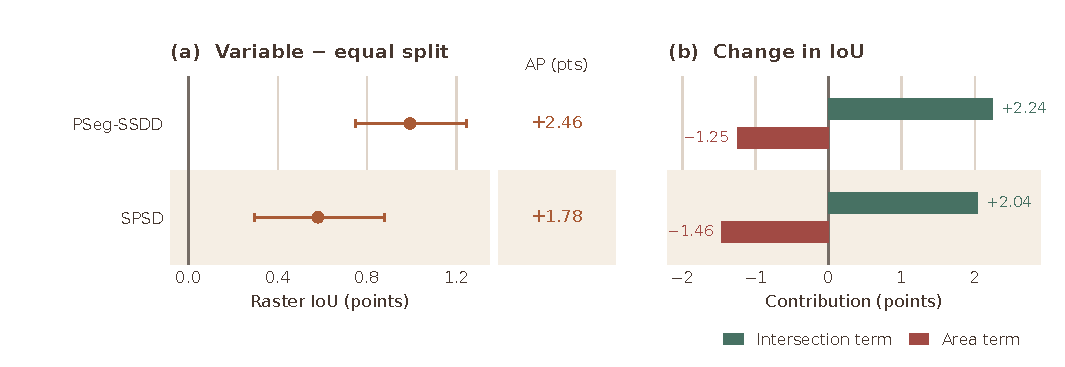
\includegraphics[width=0.98\textwidth]{figures/journal_20261126/dual_reference_budget_effect.pdf}
\caption{Fixed-total allocation for the first dual-reference ROH fit on 183 SSDD development images (115,384 flips). Both panels show variable minus equal allocation. (a) Mask AP and raster IoU under two annotations of the same images. IoU intervals are paired 95\% intervals over decoded-image groups. (b) Intersection and predicted-area contributions from Eq.~\eqref{eq:area-overlap-parts}. Table~\ref{tab:dual-sign-seeds} gives the three-fit means.}
\label{fig:dual-budget-effect}
\end{figure*}

The placement effect is smaller on PSeg-SSDD. With frozen D-FINE, \(I-L\) gains 0.021 AP and 0.069 continuous-IoU points. Excluding ten images that exactly match the historical fitting allocation leaves 222 images and gains of 0.020 and 0.072 points. Reference choice also changes the measured effect. Evaluating the same 232 images and outputs under PSeg and SPSD~\cite{slgsea}, each with its own native assignments, gives \(I-L\) all-hull raster-IoU changes of \(+0.040\) and \(-0.007\) points, respectively. The paired difference is \(-0.047\) points (\([-0.088,-0.007]\)). For natural-count editing relative to the native mask, the difference between releases is \(-0.359\) points. Edited cells that the two references label differently account for \(-0.286\) points in the common-match decomposition (Supplementary Sec.~S4).

On the 232 SAR-SSP chips, HRSID-trained RF-DETR and its scalar ROH give an \(I-F\) change of \(-0.005\) AP points. Scene-balanced raster IoU changes by \(+0.101\) points (\([-0.066,0.335]\)) over all 139 released hulls, counting a native miss as zero change. Frozen D-FINE gives \(+0.076\) AP and \(+0.022\) IoU points (\([-0.193,0.238]\)) on the same chips. Neither detector shows a clear all-hull overlap gain on this transfer.

\subsection{Signed allocation at a fixed total}
\label{sec:variable-sign-results}
At a fixed total count, moving an edit from removal to addition increases the final foreground area. We test whether that freedom improves overlap on 183 SSDD development images whose decoded-image groups were excluded from fitting. The equal and variable allocations share the D-FINE candidates, endpoint support, predicted-IoU objective and fitted dual-reference ROH. Both make 115,384 flips. The equal split adds and removes 57,692 cells each. With the first fitted head the variable split adds 67,777 and removes 47,607. All three fits improve AP and raster IoU under both annotation releases (Table~\ref{tab:dual-sign-seeds}). The releases describe the same images. Each IoU comparison retains the native assignments for its own reference, with zero change for native misses.

\begin{table}[t]
\centering
\caption{Mask AP and raster-IoU changes (points) when the addition--removal split can vary at a fixed total. The SSDD rows average three ROH fits on the same 183 images evaluated under two references. The last row evaluates the frozen policy on SAR-SSP.}
\label{tab:dual-sign-seeds}
\footnotesize
\setlength{\tabcolsep}{3.5pt}
\begin{tabular}{@{}lrl@{}}
\toprule
Evaluation reference & Mask AP & Raster IoU [95\% CI]\\
\midrule
PSeg-SSDD (183) & \(+2.299\) & \(+0.971\ [0.740,1.207]\)\\
SPSD (183) & \(+1.751\) & \(+0.573\ [0.319,0.840]\)\\
SAR-SSP (232), frozen & \(-0.139\) & \(-0.212\ [-0.547,0.104]\)\\
\bottomrule
\end{tabular}
\end{table}

The first fit gains 2.461 AP and 0.993 IoU points under PSeg and 1.782 AP and 0.580 IoU points under SPSD. To determine how much of this gain comes from covering more of the hull, let \(P_j\) denote predicted foreground area and \(I_j\) its intersection with a reference of area \(T\). Indices \(j=0\) and \(j=1\) denote equal and variable allocation. With \(U_j=P_j+T-I_j\), \(\bar P=(P_0+P_1)/2\), and \(\bar I=(I_0+I_1)/2\), the exact change in IoU is
\begin{equation}
\Delta\mathrm{IoU} =
 \frac{(\bar P+T)(I_1-I_0)-\bar I(P_1-P_0)}{U_0U_1}.
\label{eq:area-overlap-parts}
\end{equation}
The increase in intersection contributes 2.243 IoU points under PSeg and 2.041 under SPSD. The increase in predicted area costs 1.250 and 1.461 points, respectively (Fig.~\ref{fig:dual-budget-effect}). Among the 206 common positive-budget hulls, 182 gain intersection under both references and five lose intersection under at least one. Mean absolute mask-area error falls by 4.705 cells under PSeg and 1.520 under SPSD. On these images the variable split therefore recovers enough annotated hull area to outweigh the penalty for larger masks.

On 232 SAR-SSP validation chips, the frozen dual-reference head and variable allocation change 48 original matches across 20 parent scenes. Missed foreground falls by 0.653 points of reference area (\([-1.079,-0.328]\)), while excess foreground rises by 1.378 points (\([0.750,2.067]\)). Mask AP falls by 0.139 points and the raster-IoU interval spans zero. This transfer fails the paired criterion. A reference-assisted check keeps the predicted winning mask at every feasible split and uses the reference only to select the split. Across the 50 native matches with a positive budget, that choice recovers 0.958 scene-weighted IoU points on the original 139-hull denominator. The existing set of candidate edits consequently contains better allocations than the frozen policy selects. The expected-IoU and dependence checks are in Supplementary Sec.~S4.

\subsection{Where refinements recover or remove hull area}
\label{sec:qualitative}
On the historical Instance-RSDD reserve, independent ranking improves continuous IoU over bounded re-pairing for 25 of 44 eligible D-FINE matches, reduces it for 11 and leaves it unchanged for eight (Fig.~\ref{fig:rsdd-common-cap-cases}). In the positive case, the independent additions recover slightly less of the annotated hull ($-0.118$ native pixel areas). Its removals spare a further $0.711$, raising intersection by $0.593$ and IoU by $0.18$ points. In the loss case the removal terms cancel. Independent additions recover $0.875$ fewer pixel areas, and IoU falls by $0.15$ points.

\begin{figure*}[!t]
\centering
\includegraphics[width=\textwidth]{\ObservedCase{rsdd74_equal_placement.pdf}}
\caption{Independent ranking ($I$) versus bounded re-pairing ($L$) on the 74-chip Instance-RSDD reserve. The two hulls lie nearest their respective gain and loss medians among 44 eligible D-FINE matches. Both rules add and remove four cells in (a) and eight in (b). The detail enlarges the boxed region where the foreground assignments differ. Its colors distinguish $I$-only and $L$-only foreground. The right column gives whole-hull intersection changes in native pixel areas. A positive removal term means that $I$ removes less of the annotated hull. Among $4\times4$ windows on the display grid, the box encloses the largest GT area on which the two masks disagree. \CaseCaption{Each full view pools GT or mask coverage on an $8\times8$ grid. Dashed contours mark 50\% GT coverage. The detail shows the mean signed foreground difference per bin.}{The masks and GT polygon share the same native SAR crop. Dashed contours trace the GT polygon and solid contours the predicted mask.} Changes use unrounded values.}
\label{fig:rsdd-common-cap-cases}
\end{figure*}

The HRSID DEV705 examples show how additions and removals contribute separately. Both methods make eight swaps. In the positive case, independent selection recovers one more pixel-equivalent of the reference polygon through additions and spares a further 1.5 through removals compared with distance-first pairing. IoU rises by 0.732 points. In the negative case, neither method's additions intersect the reference, but independent selection removes one additional pixel-equivalent of the hull. IoU falls by 0.316 points. A lower predicted occupancy can therefore send the writer to a cell that contains more of the annotated hull.

At the dynamic-attraction budget on Gaofen-3, ROH ranking improves 268 of 425 eligible RF-DETR matches, worsens 154 and ties three (Fig.~\ref{fig:gf3-qual}). In the gain case, better-placed additions recover $2.467$ more native pixel areas of the GT hull and removals spare another $1.245$. Intersection increases by $3.71$ in total and IoU rises from $71.86$ to $72.56$. In the loss case the additions contribute the same intersection. ROH removes three more native pixel areas of the hull, and IoU falls from $68.14$ to $67.58$. Supplementary Section~S5 includes the two other matched examples.

\begin{figure*}[!t]
\centering
\includegraphics[width=\textwidth]{\ObservedCase{gf3_matched_ranking.pdf}}
\caption{ROH ranking versus dynamic attraction on Gaofen-3 with frozen RF-DETR fit B. Each rule makes eight additions and eight removals per case. From two near-median gains and two near-median losses, the example of each sign with the larger absolute change in intersection is shown. The crop and edit count are fixed within each row. The detail enlarges the boxed region and shows the signed change in GT intersection, ROH minus attraction. The right column separates the whole-hull change into contributions from additions and removals. Among $4\times4$ windows on the display grid, the box encloses the largest GT area on which the two masks disagree. \CaseCaption{GT coverage is averaged on an $8\times8$ grid, and a dashed line marks the 50\% contour. Predicted mask coverage uses quarter levels. Detail bins sum signed polygon--cell intersection changes in native pixel areas.}{Dashed contours trace the GT polygon and solid contours the predicted mask in the registered SAR crop.} Changes use unrounded values.}
\label{fig:gf3-qual}
\end{figure*}

The whole-crop comparison exposes a different failure mode (Fig.~\ref{fig:retained-whole-cases}). On the narrow hull in (a), local ROH keeps the lower end close to the native outline. SegRefiner-LR retracts the mask, and its IoU falls to 67.43 compared with 71.95 for ROH and 71.93 for the native mask. In (b), the native mask extends beyond the annotated hull. Whole-crop refinement trims the extension and reaches 60.96, compared with 58.89 for ROH and 58.68 for the native mask. Both the number and the locations of the edits differ, so the IoU gaps describe the complete mask updates.

\begin{figure*}[!t]
\centering
\includegraphics[width=\textwidth]{\ObservedCase{retained_hulls.pdf}}
\caption{Local ROH and whole-crop SegRefiner-LR on two Instance-RSDD reserve detections. Cases lie nearest the median loss (a) and gain (b) for SegRefiner-LR relative to the native mask among 39 gate-exposed matches. Labels give continuous IoU on the same polygon and the difference between the two refined masks, in points. The two writers have different edit support and counts. \CaseCaption{Mask coverage is pooled on an \(8\times8\) display grid. The dashed contour marks 25\% GT coverage.}{The solid boundary follows the prediction on the registered SAR crop, and the dashed outline is the GT polygon.} Boxes mark the same detail window across each row.}
\label{fig:retained-whole-cases}
\end{figure*}

\subsection{Ablations and alternative rankers}
\label{sec:ablation}

\textit{Addition and removal locations.}
Holding the ROH scores, candidate cells and both signed counts at their \(F\) values, we switch the addition sites, the removal sites or both to independent ranks. Switching either side alone increases AP, and switching both gives the highest AP in every row of Table~\ref{tab:signed-side-ablation}. On Gaofen-3 the extra gain from switching both sides averages 0.224 AP and 0.175 continuous-IoU points (\([0.130,0.222]\) for IoU) over switching additions alone, and 0.199 AP and 0.085 IoU points (\([0.049,0.120]\)) over switching removals alone. The corresponding IoU gains on the 74-chip reserve are 0.170 and 0.148 points, with both intervals above zero. Because mask area is fixed, the geometric comparison measures the choice of sites. AP can also change when score-ordered predictions are rematched.

\begin{table}[t]
\centering
\caption{Mask AP when independent ranks replace paired locations for additions, removals or both. Per-side counts stay fixed. The two Gaofen-3 fits share the detector and images.}
\label{tab:signed-side-ablation}
\footnotesize
\setlength{\tabcolsep}{3.5pt}
\begin{tabular}{@{}lrrrr@{}}
\toprule
Instance-RSDD view & Paired & Add & Remove & Both\\
\midrule
Gaofen-3, first ROH & 61.036 & 61.331 & 61.286 & 61.518\\
Gaofen-3, second ROH & 60.984 & 61.207 & 61.302 & 61.468\\
Reserve (74) & 58.278 & 58.545 & 58.426 & 58.714\\
Date-separated (42) & 61.283 & 61.769 & 61.698 & 62.123\\
\bottomrule
\end{tabular}
\end{table}

\textit{Scoring under a shared attraction budget.}
Can a spatial rule rank the same candidate cells as effectively as ROH? At the dynamic-attraction count on HRSID DEV705, ROH, dynamic attraction and static attraction each make 262,802 swaps and score 50.727, 48.299 and 48.396 AP, respectively. ROH gains 1.150 continuous-IoU points over dynamic attraction across 1,447 fixed matches in 27 source-prefix groups (\([0.927,1.397]\)). With counts matched within each target cohort, ROH gains 0.468 AP and 0.431 IoU points (\([0.213,0.662]\)) on the 74-chip reserve, but loses 0.026 AP and 0.270 IoU points (\([-0.440,-0.098]\)) on the 232 PSeg-SSDD images.

The choice of training target also affects the measured advantage of ROH. On D-FINE FIT109, fractional occupancies give a 0.184-point AP gain over COCO raster targets. The gain falls to 0.051 AP points against targets hardened at 0.50, with a loss in one fit. Supplementary Sec.~S6 gives the alternative target, capacity and feature controls.

\textit{PointRend under matched support and counts.}
We adapt PointRend~\cite{pointrend} to frozen RF-DETR features from FIT109 and compare it with ROH first as a ranker, then as a whole-RoI refiner (Table~\ref{tab:rsdd-pointrend}). With identical signed counts and capped candidate sites on Gaofen-3, ROH gains 0.312 AP and 0.250 continuous-IoU points (\([0.163,0.338]\)) over PointRend. With complete two-ring support the gains are 0.390 AP and 0.223 IoU points (\([0.123,0.330]\)). At 31,391 matched exchanges on capped support on the historical reserve, ROH gains 0.477 AP and 0.395 IoU points (\([0.204,0.620]\)). The reserve one-pixel Boundary-IoU interval spans zero.

Giving PointRend its own whole-RoI paste changes the candidate sites and counts. On Gaofen-3 it reaches 61.831 AP compared with 61.631 for ROH on complete two-ring support. Their AR100 values are 72.361 and 74.105, respectively. A partial substitution keeps PointRend's signed counts and its paste outside the sampled cells, using ROH ranks only inside. This raises mean AP from 61.831 to 61.975 on Gaofen-3 and from 57.534 to 58.196 on the reserve. These results apply to the adapted head and tested detector streams.

\begin{table}[t]
\centering
\caption{Gaofen-3 scores for native masks, whole-RoI pastes and ranking on matched support. Within each matched pair, both rankers make 268,347 exchanges. Continuous IoU weights acquisitions equally over 425 fixed matches.}
\label{tab:rsdd-pointrend}
\setlength{\tabcolsep}{4pt}
\begin{tabular}{lrrrr}
\toprule
Policy & AP & AP75 & AP90 & IoU\\
\midrule
Native RF-DETR & 61.033 & 71.822 & 3.256 & 79.652\\
Coarse RoI paste & 53.880 & 56.474 & 1.486 & 75.108\\
PointRend RoI paste & 61.831 & 74.396 & 3.227 & 79.939\\
\midrule
PointRend ranks, capped & 61.309 & 72.646 & 3.017 & 79.647\\
ROH ranks, capped & 61.620 & 73.259 & 3.162 & 79.897\\
PointRend ranks, complete & 61.241 & 72.525 & 3.015 & 79.648\\
ROH ranks, complete & 61.631 & 73.280 & 3.041 & 79.871\\
\bottomrule
\end{tabular}
\end{table}

\textit{Frozen general refiners.}
With the fifth-iteration probabilities and candidates of Phoenix XL1~\cite{phoenix} fixed, replacing whole-grid thresholding with an exact count reduces the edits from 2,042,908 to 59,800 flips on the reserve and from 3,391,327 to 147,540 on PSeg-SSDD. AP rises from 49.085 to 58.478 and from 13.922 to 16.447, respectively. Continuous IoU gains 9.462 (\([6.329,13.283]\)) and 4.001 (\([2.644,5.382]\)) points. Restricting the support at those same counts has different effects on the two cohorts, \(+0.281\) and \(-0.323\) IoU points. In a separate comparison on the reserve, we disable the Phoenix \(1\%\) gate and match its candidate cells and signed counts to ROH. Phoenix leads by 0.308 AP points, with an uncertain continuous-IoU difference.

Whole-crop writing with the released COCO SegRefiner-LR checkpoint~\cite{segrefiner}, its original area gate and six denoising steps gives 56.574 AP on the reserve and 17.136 on PSeg-SSDD. Both fall below the corresponding native scores of 58.277 and 17.974. Separating the original deletions from the additions shows continuous-IoU losses of about four points on the 39 and 67 gate-exposed matches, respectively. Supplementary Section~S4-F gives the checkpoint and eligibility details for both refiners. Section~S6-C examines writable support and edit count for Phoenix.

\textit{Limits of the detection box.}
A reference-guided check isolates errors imposed by the original detection box. Among 1,329 small, elongated D-FINE matches on HRSID DEV705, expanding the box by two pixels on each side makes continuous IoU above 0.90 attainable for 134 cases previously blocked by the box. None reaches that level by adding foreground in the new strip alone. At least 91 also require additional foreground inside the original box and removal of some original foreground.

\textit{Writing time on cached inputs.}
With scores, candidate sites and counts cached, distance-first pairing, bounded re-pairing and independent selection take 26.1, 138.6 and 27.4\,ms per image on the same single CPU thread, including run-length encoding. Supplementary Sec.~S7 reports timings for the scoring and decoding paths separately.

\section{Discussion}
\label{sec:discussion}

When a boundary update must preserve foreground area, every gain in continuous IoU comes from a gain in intersection with the reference. This observation explains why a useful edit need not exchange adjacent cells. On the historical reserve, re-pairing cells within the original distance cap improves agreement in the one-pixel boundary band. Removing the cap improves whole-mask overlap and AP with two frozen pipelines on the same chips. Whether lifting it further improves the narrow band remains unresolved. The loss examples show the practical limit of independent selection. The best-ranked cell can contain less of the annotated hull than its alternative.

Which cells can be edited also matters when interpreting a comparison between refiners. The same-site comparisons with attraction and adapted PointRend test the ordering of cells. PointRend's whole-RoI comparison allows it to change additional sites, and its AP advantage on Gaofen-3 coexists with a ROH advantage on matched sites. Likewise, constraining the Phoenix flip count helps on both tested cohorts on the full grid, whereas narrowing its support helps on only one cohort. Fractional targets provide a way to score partially annotated cells. How much this supervision helps depends on the raster or thresholded target used for comparison.

Relaxing the balance between additions and removals changes what a correction can accomplish. On SSDD, added foreground covers enough of the annotated hull to improve overlap under both releases and across repeated fits. Those releases are two annotations of the same images, and refitting the head leaves those evaluation images fixed. On SAR-SSP, the same policy recovers missed foreground but includes more background and lowers mask AP. The reference-assisted split check shows that useful edits were available even where the frozen allocation failed. It leaves open how to identify those edits from the target image and frozen scores alone.

The retained detection sets an outer limit on each result. When the mask and its writable region miss a vessel, a local update cannot recover it. The expanded-box check shows why merely reaching more cells can be insufficient. Some masks need both new foreground inside the original box and removal of existing foreground. Preserving area alone gives no guarantee of a connected hull, and overlap with an annotation has a different meaning from accuracy in physical length. The historical exposure and nested sensor--date screens limit the independence of the transfer evidence. Supplementary Secs.~S4 and S7 detail acquisition and exposure, topology, physical-length checks and timing. The prospective Umbra views await independent outline scoring.

The placement rules differ in computational cost even after the scores are available. Bounded re-pairing searches over competing assignments within a distance cap, a more expensive step in the cached single-thread replay than either distance-first pairing or independent selection. This comparison isolates the cost of writing a mask from prepared inputs.

\section{Conclusion}
NORA ranks candidate boundary cells by estimated polygon coverage to choose where to edit. Its dual-reference variant learns foreground probabilities from two raster annotations to divide a fixed number of edits between additions and removals. With candidate cells, scores and per-side counts held fixed, independent ranking improves whole-mask overlap and mask AP on HRSID and selected frozen Instance-RSDD views. Bounded re-pairing provides the clearest gain at the one-pixel boundary on the historical reserve. Allowing additions to outnumber removals recovers more annotated hull area on the SSDD development images under both references. On SAR-SSP the same frozen allocation adds excess foreground and reduces AP. The benefit of changing an edit rule therefore depends on which cells the detector makes available and how accurately their scores predict coverage under the target reference.
\par\label{main:body:end}

\section*{Data and Code Availability}
The \href{https://github.com/bingzhi495-creator/SAR-SEAL-research}{project repository} provides analysis code, configurations, evaluation protocols, aggregate results and links to the data releases. The \href{https://github.com/bingzhi495-creator/SAR-SEAL-research/blob/main/research_round_20260925_global/paper_boundary_refinement_20261120/design/NORA_REPRODUCIBILITY.md}{reproducibility index} identifies the frozen detector and ROH fits, splits, and capture and replay procedures for the fixed-mask comparisons. Images and reference outlines are available under the terms of their respective releases.

\ifnativecases\IEEEtriggeratref{17}\else\IEEEtriggeratref{15}\fi
\begin{thebibliography}{22}
\bibitem{moreira2013} A. Moreira, P. Prats-Iraola, M. Younis, G. Krieger, I. Hajnsek, and K. P. Papathanassiou, ``A tutorial on synthetic aperture radar,'' \emph{IEEE Geosci. Remote Sens. Mag.}, vol. 1, no. 1, pp. 6--43, 2013. \href{https://doi.org/10.1109/MGRS.2013.2248301}{10.1109/MGRS.2013.2248301}.
\bibitem{gao2024} F. Gao, X. Han, J. Wang, J. Sun, A. Hussain, and H. Zhou, ``SAR ship instance segmentation with dynamic key points information enhancement,'' \emph{IEEE J. Sel. Topics Appl. Earth Observ. Remote Sens.}, vol. 17, pp. 11365--11385, 2024. \href{https://doi.org/10.1109/JSTARS.2024.3383779}{10.1109/JSTARS.2024.3383779}.
\bibitem{gldet} H. Chang, X. Fu, P. Lang, K. Guo, J. Dong, and S. Chang, ``GLDet: Real-time SAR ship detector based on global semantic information enhancement and local gradient information mining,'' \emph{IEEE Trans. Geosci. Remote Sens.}, vol. 63, Art. no. 5209020, 2025. \href{https://doi.org/10.1109/TGRS.2025.3559551}{10.1109/TGRS.2025.3559551}.
\bibitem{hrsid} S. Wei, X. Zeng, Q. Qu, M. Wang, H. Su, and J. Shi, ``HRSID: A high-resolution SAR images dataset for ship detection and instance segmentation,'' \emph{IEEE Access}, vol. 8, pp. 120234--120254, \href{https://doi.org/10.1109/ACCESS.2020.3005861}{2020}.
\bibitem{ssdd} T. Zhang \emph{et al.}, ``SAR Ship Detection Dataset (SSDD): Official release and comprehensive data analysis,'' \emph{Remote Sens.}, vol. 13, no. 18, Art. no. 3690, 2021. \href{https://doi.org/10.3390/rs13183690}{10.3390/rs13183690}.
\bibitem{boundaryiou} B. Cheng, R. Girshick, P. Doll{\'a}r, A. C. Berg, and A. Kirillov, ``Boundary IoU: Improving object-centric image segmentation evaluation,'' in \emph{Proc. IEEE/CVF Conf. Comput. Vis. Pattern Recognit. (CVPR)}, 2021. \href{https://arxiv.org/abs/2103.16562}{arXiv:2103.16562}.
\bibitem{rsdd} X. Yang, Q. Zhang, Q. Dong, Z. Han, X. Luo, and D. Wei, ``Ship instance segmentation based on rotated bounding boxes for SAR images,'' \emph{Remote Sens.}, vol. 15, no. 5, Art. no. 1324, \href{https://doi.org/10.3390/rs15051324}{2023}.
\bibitem{drsnet} Q. Zhang and Z. Han, ``DRSNet: Rotated-ROI ship segmentation for SAR images based on dual-scale cross attention,'' \emph{IEEE Geosci. Remote Sens. Lett.}, vol. 21, pp. 1--5, 2024. \href{https://doi.org/10.1109/LGRS.2024.3420251}{10.1109/LGRS.2024.3420251}.
\bibitem{aranet} S. Chang, P. Lang, H. Chang, C. Zhao, J. Yang, J. Dong, and X. Fu, ``ARANet: A unified representation alignment framework for SAR ship instance segmentation,'' \emph{IEEE J. Sel. Topics Appl. Earth Observ. Remote Sens.}, vol. 19, pp. 28679--28694, 2026. \href{https://doi.org/10.1109/JSTARS.2026.3720719}{10.1109/JSTARS.2026.3720719}.
\bibitem{dacf} S. Yang, X. Zhang, W. An, Z. Li, and N. Chen, ``DACF-Net: A dynamic attention and context fusion network with geometry-aware multi-scale refinement for SAR ship instance segmentation,'' \emph{Int. J. Digit. Earth}, vol. 19, no. 2, Art. no. 2696657, 2026. \href{https://doi.org/10.1080/17538947.2026.2696657}{10.1080/17538947.2026.2696657}.
\bibitem{dsr} S.-W. He, W. Xiong, and L.-B. Yao, ``SAR ship instance segmentation method in complex scenes jointly driven by differential physical fields and structured graph reasoning,'' \emph{Acta Electronica Sinica}, pp. 1--11, 2026. \href{https://doi.org/10.12263/DZXB.20260699}{10.12263/DZXB.20260699}.
\bibitem{atkinson} P. M. Atkinson, ``Sub-pixel target mapping from soft-classified, remotely sensed imagery,'' \emph{Photogramm. Eng. Remote Sens.}, vol. 71, no. 7, pp. 839--846, 2005. \href{https://doi.org/10.14358/PERS.71.7.839}{10.14358/PERS.71.7.839}.
\bibitem{pointrend} A. Kirillov, Y. Wu, K. He, and R. Girshick, ``PointRend: Image segmentation as rendering,'' in \emph{Proc. IEEE/CVF Conf. Comput. Vis. Pattern Recognit. (CVPR)}, 2020, pp. 9799--9808.
\bibitem{segfix} Y. Yuan, J. Xie, X. Chen, and J. Wang, ``SegFix: Model-agnostic boundary refinement for segmentation,'' in \emph{Proc. Eur. Conf. Comput. Vis. (ECCV)}, 2020, pp. 489--506.
\bibitem{bpr} C. Tang, H. Chen, X. Li, J. Li, Z. Zhang, and X. Hu, ``Look closer to segment better: Boundary patch refinement for instance segmentation,'' in \emph{Proc. IEEE/CVF Conf. Comput. Vis. Pattern Recognit. (CVPR)}, 2021, pp. 13926--13935.
\bibitem{rankseg} B. Dai and C. Li, ``RankSEG: A consistent ranking-based framework for segmentation,'' \emph{J. Mach. Learn. Res.}, vol. 24, no. 224, pp. 1--50, \href{https://www.jmlr.org/papers/v24/22-0712.html}{2023}.
\bibitem{rankrma} Z. Wang and B. Dai, ``RankSEG-RMA: An efficient segmentation algorithm via reciprocal moment approximation,'' in \emph{Adv. Neural Inf. Process. Syst.}, vol. 38, 2025. \href{https://doi.org/10.52202/085713-5452}{10.52202/085713-5452}.
\bibitem{segrefiner} M. Wang, H. Ding, J. H. Liew, J. Liu, Y. Zhao, and Y. Wei, ``SegRefiner: Towards model-agnostic segmentation refinement with discrete diffusion process,'' in \emph{Adv. Neural Inf. Process. Syst.}, vol. 36, 2023. \href{https://proceedings.neurips.cc/paper_files/paper/2023/hash/fc0cc55dca3d791c4a0bb2d8ddeefe4f-Abstract-Conference.html}{Proceedings}.
\bibitem{phoenix} B. Kim and S. J. Hwang, ``Learning from adversity: Semantic-aware mask refinement through adversarial perturbation,'' in \emph{Proc. Eur. Conf. Comput. Vis. (ECCV)}, 2026, pp. 75--92. \href{https://doi.org/10.1007/978-3-032-37520-9_5}{10.1007/978-3-032-37520-9\_5}.
\bibitem{rfdetr} I. Robinson, P. Robicheaux, M. Popov, D. Ramanan, and N. Peri, ``RF-DETR: Neural architecture search for real-time detection transformers,'' in \emph{Proc. Int. Conf. Learn. Represent. (ICLR)}, 2026.
\bibitem{dfine} A. Saakyan and D. Solntsev, ``D-FINE-seg: Object detection and instance segmentation framework with multi-backend deployment,'' \href{https://arxiv.org/abs/2602.23043}{arXiv:2602.23043}, 2026.
\bibitem{slgsea} R. Deng, T. Zhang, G. Gao, L. Zhang, S. Wei, and X. Zhang, ``SLGSea: Spatialized language guidance with scattering-aware query construction for ship--sea--land panoptic segmentation in SAR imagery,'' project repository and dataset release. \href{https://github.com/deng1218/SLGSea}{Code and data}.
\end{thebibliography}
\end{document}
